% Documentación de la Etapa 3
% Compilar con:  pdflatex Informe_etapa3.tex
\documentclass[11pt,a4paper]{article}

\usepackage[utf8]{inputenc}
\usepackage[margin=2.5cm]{geometry}
\usepackage{url}
\usepackage{graphicx}
\usepackage{tikz}

\title{Etapa 3 - Analizador Semántico (Chequeo de Declaraciones) de MiniJava}
\author{Compiladores e Intérpretes --- UNS, 2026}
\date{}

% Esta instalacion TeX puede no tener las fuentes TS1 (text companion): se evitan
% los simbolos que las requieren (vinetas de itemize, llaves via \{ en \texttt).
\renewcommand{\labelitemi}{$\bullet$}

\begin{document}

\sloppy

\maketitle

\noindent
Implementación del chequeo de declaraciones del analizador semántico de MiniJava.
Se extiende el analizador sintáctico descendente recursivo de la Etapa 2 para que
construya la Tabla de Símbolos (TS) a medida que reconoce las declaraciones, y se
agrega una segunda pasada de control de declaraciones y la consolidación de clases
e interfaces. No se chequean los cuerpos de métodos ni de constructores: esos
controles corresponden a la Etapa 4.

\section{Objetivo y logros}

\begin{itemize}
  \item Construir y consolidar la TS global de tipos, con las clases e interfaces
        declaradas y las entidades predefinidas.
  \item Controlar la correctitud de todas las declaraciones (nombres repetidos,
        tipos válidos, relaciones de herencia, circularidad, redefiniciones y
        contratos de interfaces).
  \item Reportar el primer error con un mensaje descriptivo y el código
        \texttt{[Error:lexema|nroLinea]}, o \texttt{[SinErrores]} si el programa
        es válido.
\end{itemize}

Se implementan los logros de la etapa anterior que siguen vigentes (atributos
inicializados, operadores posfijos y visibilidad mejorada) y el manejo de archivos
eficiente. No se implementan los logros opcionales de la Etapa 3 (modificadores
\texttt{sealed}/\texttt{final}, herencia múltiple de interfaces ni métodos
genéricos), que requieren extender el léxico y la gramática.

\section{Esquema general}

El módulo principal recibe el archivo fuente y lo asocia al manejador de archivos y
este al léxico. Luego crea la \texttt{TablaDeSimbolos} (que ya carga \texttt{Object},
\texttt{String} y \texttt{System}) y el \texttt{AnalizadorSintactico} con dependencia
al léxico y a la TS. El sintáctico, mientras valida la sintaxis, ejecuta las acciones
semánticas que insertan las entidades en la TS y realizan los controles de la primera
pasada. Al finalizar el parseo, el módulo principal ejecuta el chequeo de
declaraciones (\texttt{estaBienDeclarada}) y la consolidación (\texttt{consolidar}).
Si no hay errores informa el mensaje de éxito; ante un error léxico, sintáctico o
semántico captura la excepción correspondiente, reporta el mensaje y el código de
error, y finaliza la ejecución.

\begin{figure}[h]
\centering
\resizebox{\textwidth}{!}{%
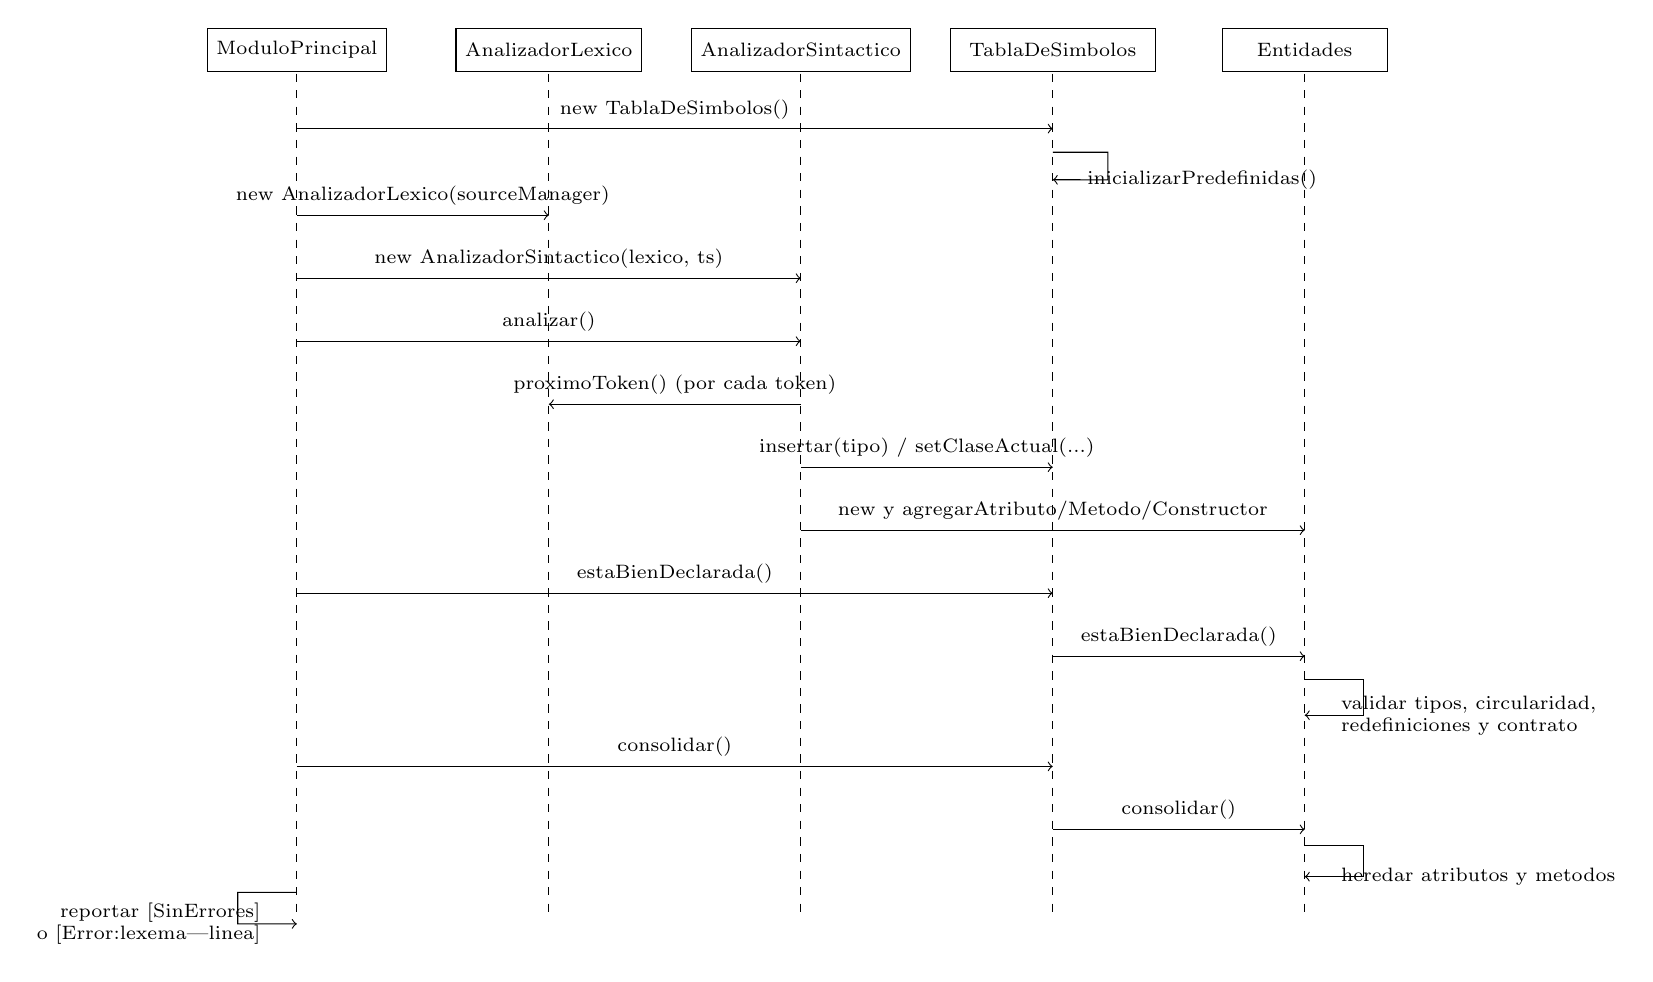
\begin{tikzpicture}[font=\scriptsize]
\def\MP{0}\def\AL{3.2}\def\AS{6.4}\def\TS{9.6}\def\EN{12.8}
% participantes
\node[draw,minimum width=2.2cm,minimum height=0.55cm] (mp) at (\MP,0) {ModuloPrincipal};
\node[draw,minimum width=2.3cm,minimum height=0.55cm] (al) at (\AL,0) {AnalizadorLexico};
\node[draw,minimum width=2.6cm,minimum height=0.55cm] (as) at (\AS,0) {AnalizadorSintactico};
\node[draw,minimum width=2.6cm,minimum height=0.55cm] (ts) at (\TS,0) {TablaDeSimbolos};
\node[draw,minimum width=2.1cm,minimum height=0.55cm] (en) at (\EN,0) {Entidades};
% lineas de vida
\foreach \x in {\MP,\AL,\AS,\TS,\EN} { \draw[dashed] (\x,-0.3) -- (\x,-11.0); }
% mensajes
\draw[->] (\MP,-1.0) -- (\TS,-1.0) node[midway,above,align=center]{new TablaDeSimbolos()};
\draw[->] (\TS,-1.3) -- ++(0.7,0) -- ++(0,-0.35) -- (\TS,-1.65)
    node[right,align=left,pos=0.55]{inicializarPredefinidas()};
\draw[->] (\MP,-2.1) -- (\AL,-2.1) node[midway,above,align=center]{new AnalizadorLexico(sourceManager)};
\draw[->] (\MP,-2.9) -- (\AS,-2.9) node[midway,above,align=center]{new AnalizadorSintactico(lexico, ts)};
\draw[->] (\MP,-3.7) -- (\AS,-3.7) node[midway,above,align=center]{analizar()};
\draw[->] (\AS,-4.5) -- (\AL,-4.5) node[midway,above,align=center]{proximoToken() (por cada token)};
\draw[->] (\AS,-5.3) -- (\TS,-5.3) node[midway,above,align=center]{insertar(tipo) / setClaseActual(...)};
\draw[->] (\AS,-6.1) -- (\EN,-6.1) node[midway,above,align=center]{new y agregarAtributo/Metodo/Constructor};
\draw[->] (\MP,-6.9) -- (\TS,-6.9) node[midway,above,align=center]{estaBienDeclarada()};
\draw[->] (\TS,-7.7) -- (\EN,-7.7) node[midway,above,align=center]{estaBienDeclarada()};
\draw[->] (\EN,-8.0) -- ++(0.75,0) -- ++(0,-0.45) -- (\EN,-8.45)
    node[right,align=left,pos=0.55]{validar tipos, circularidad,\\redefiniciones y contrato};
\draw[->] (\MP,-9.1) -- (\TS,-9.1) node[midway,above,align=center]{consolidar()};
\draw[->] (\TS,-9.9) -- (\EN,-9.9) node[midway,above,align=center]{consolidar()};
\draw[->] (\EN,-10.1) -- ++(0.75,0) -- ++(0,-0.4) -- (\EN,-10.5)
    node[right,align=left,pos=0.55]{heredar atributos y metodos};
\draw[->] (\MP,-10.7) -- ++(-0.75,0) -- ++(0,-0.4) -- (\MP,-11.1)
    node[left,align=right,pos=0.55]{reportar [SinErrores]\\o [Error:lexema|linea]};
\end{tikzpicture}%
}
\caption{Diagrama de secuencia del análisis de la Etapa 3.}
\end{figure}

\section{Estructura del proyecto}

{\footnotesize
\begin{verbatim}
compilador-minijava/
|-- Compilar.sh / Compilar.bat          Compila y genera Compilador.jar
|-- CorrerTests.sh / CorrerTests.bat    Compila y ejecuta los testers JUnit
|-- lib/                                Jars de JUnit 4 y Hamcrest (se autodescargan)
|-- src/main/java/
|   |-- moduloprincipal/
|   |   \-- ModuloPrincipal.java        Modulo principal (interfaz con el usuario)
|   |-- analizadorlexico/               Etapa 1 (sin cambios)
|   |-- analizadorsintactico/
|   |   |-- AnalizadorSintactico.java   Parser + acciones semanticas (construye la TS)
|   |   \-- ExcepcionSintactica.java    Error sintactico
|   |-- analizadorsemantico/            NUEVO: Tabla de Simbolos y chequeos
|   |   |-- TablaDeSimbolos.java        Tabla global, predefinidas, puntos de entrada
|   |   |-- Entidad.java                Entidad declarable (abstracta)
|   |   |-- Clase.java                  Clase concreta
|   |   |-- Interfaz.java               Interfaz
|   |   |-- Metodo.java                 Metodo
|   |   |-- Constructor.java            Constructor
|   |   |-- Atributo.java               Atributo de instancia
|   |   |-- Parametro.java              Parametro formal
|   |   |-- Tipo.java                   Tipo (abstracto)
|   |   |-- TipoPrimitivo.java          boolean / char / int
|   |   |-- TipoVoid.java               void (solo retorno)
|   |   |-- TipoParametro.java          Parametro de tipo (T)
|   |   |-- TipoArreglo.java            Arreglo con dimensiones
|   |   |-- TipoReferencia.java         Clase/interfaz con argumento generico opcional
|   |   \-- ExcepcionSemantica.java     Error semantico
|   \-- sourcemanager/                  Etapa 1 (sin cambios)
|-- src/test/java/test/                 Testers JUnit provistos por la catedra
\-- resources/
    |-- sinErrores/                     Casos de prueba sin errores
    \-- conErrores/                     Casos de prueba con errores
\end{verbatim}
}

\section{Tabla de símbolos}

Cada entidad declarable se representa con una clase que conserva el token de su
declaración (lexema y número de línea) y sabe controlarse a sí misma. La tabla
global comparte el espacio de nombres de clases e interfaces y mantiene las clases
predefinidas.

\subsection{Diagrama de clases}

{\footnotesize
\begin{verbatim}
                         +---------------------------+
                         |      TablaDeSimbolos      |
                         +---------------------------+
                         | - clases: Map<String,     |
                         |          Clase>           |
                         | - interfaces: Map<String, |
                         |          Interfaz>        |
                         | - claseActual: Clase      |
                         | - interfazActual: Interfaz|
                         | - metodoActual: Metodo    |
                         +---------------------------+
                         | + insertar(e)             |
                         | + esTipo(n) / getTipo(n)  |
                         | + estaBienDeclarada()     |
                         | + consolidar()            |
                         +-------------+-------------+
                                       | 1..*
                                       v
                         +---------------------------+
                         |        <<Entidad>>        |
                         +---------------------------+
                         | # token: Token            |
                         | # nombre: String          |
                         +---------------------------+
                         | + estaBienDeclarada()     |
                         | + getParametroGenerico()  |
                         +-------------+-------------+
                    ______________|______________
                   /              |              \
                  v               v               v
        +----------------+ +--------------+ +----------------+
        |     Clase      | |  Interfaz    | |    Metodo      |
        +----------------+ +--------------+ +----------------+
        | - parametroGen | | - parametroG | | - tipoRetorno  |
        | - herencia     | | - ancestro   | | - params{}     |
        | - ancestroEsI? | | - metodos{}  | | - esEstatico   |
        | - atributos{}  | +--------------+ +----------------+
        | - metodos{}    | | + estaBien.. | | + getClave()   |
        | - constructores| | + checkCirc..| | + mismaFirma() |
        +----------------+ +--------------+ +-------+--------+
        | + estaBien..   |                        | 0..*
        | + consolidar   |                        v
        +---+-------+----+              +----------------+
            |       |                   |   Parametro    |
            | 0..1  | 0..*              +----------------+
            v       v                   | - tipo: Tipo   |
      +----------+ +--------------+     | - posicion:int |
      | Atributo | | Constructor  |     +----------------+
      +----------+ +--------------+     | + estaBien..   |
      | - tipo   | | - params{}   |     +----------------+
      +----------+ +--------------+

                         +---------------------------+
                         |         <<Tipo>>          |
                         +---------------------------+
                         | # token: Token            |
                         +---------------------------+
                         | + esValidoEn(ts,c)        |
                         | + sustituir(map)          |
                         | + esIgualA(t)             |
                         +-------------+-------------+
             __________________________|__________________________
            /            /                    \                  \
           v            v                      v                  v
   +-------------+ +----------+     +-----------------+  +----------------+
   |TipoPrimitivo| | TipoVoid |     | TipoParametro   |  | TipoArreglo    |
   +-------------+ +----------+     +-----------------+  +----------------+
                                                           | - base, dims
   +------------------+                                    +----------------+
   | TipoReferencia   |
   | - nombre         |
   | - argumento (opt)|
   +------------------+
\end{verbatim}
}

\subsection{Responsabilidades}

\begin{itemize}
  \item \texttt{TablaDeSimbolos}: administra el espacio global de tipos, las
        entidades predefinidas y el contexto actual; recorre la tabla para el
        chequeo y la consolidación.
  \item \texttt{Clase}/\texttt{Interfaz}: controlan su relación de herencia, su
        circularidad, sus tipos y sus miembros; consolidan su tabla respectiva.
  \item \texttt{Metodo}/\texttt{Constructor}/\texttt{Atributo}/\texttt{Parametro}:
        controlan la validez de sus tipos y de sus nombres.
  \item \texttt{Tipo} y sus subclases: modelan de forma uniforme los tipos
        primitivos, \texttt{void}, parámetros de tipo, arreglos y referencias con
        argumento genérico; implementan validez, sustitución e igualdad estructural.
\end{itemize}

\section{Chequeo de declaraciones}

\subsection{Primera pasada (construcción de la TS)}

Se ejecuta durante el parseo, al insertar cada entidad. Controla:

\begin{itemize}
  \item nombres de tipo repetidos (y redeclaración de \texttt{Object},
        \texttt{String} y \texttt{System}, que ya están en la tabla);
  \item dos atributos con el mismo nombre en una clase;
  \item dos métodos con la misma clave \texttt{(nombre, aridad)} en una clase o
        interfaz, aunque difieran en los tipos o nombres de sus parámetros;
  \item dos constructores con la misma aridad en una clase;
  \item parámetros repetidos en una misma unidad (método o constructor);
  \item que el nombre de cada constructor coincida con el de su clase.
\end{itemize}

\subsection{Segunda pasada (\texttt{estaBienDeclarada})}

Se ejecuta una vez finalizado el parseo. Controla:

\begin{itemize}
  \item que todo tipo referencia usado en atributos, retornos y parámetros exista
        (clase, interfaz o entidad predefinida);
  \item que el argumento genérico sea válido: el tipo referenciado debe declarar un
        parámetro de tipo y el argumento debe ser un parámetro de tipo válido en el
        contexto o un tipo existente;
  \item que un parámetro de tipo solo se use dentro de la clase o interfaz que lo
        declara;
  \item que \texttt{extends} apunte a una clase existente, \texttt{implements} a una
        interfaz existente y la extensión de interfaz a otra interfaz;
  \item la ausencia de herencia circular entre clases y de extensión circular entre
        interfaces;
  \item la redefinición de métodos de instancia (mismo nombre y aridad que un método
        heredado exige signaturas exactamente iguales: misma cantidad, mismos tipos
        de parámetros en orden y mismo retorno, tras instanciar los genéricos);
  \item los conflictos con métodos estáticos heredados (un método estático heredado
        con una clave prohíbe cualquier método con esa clave, estático o de
        instancia, y un método estático nuevo no puede chocar con un método de
        instancia heredado);
  \item el contrato de interfaces: la clase debe poseer, directa o heredadamente, un
        método de instancia compatible con cada método de la interfaz (un método
        estático no la implementa).
\end{itemize}

\subsection{Consolidación}

La consolidación incorpora los miembros heredados con delegación y recursión: una
clase se consolida solo después de su ancestro directo. Al heredar de un tipo
genérico, los tipos paramétricos de los miembros heredados se instancian con el
argumento explícito (por ejemplo \texttt{extends A<String>}) o conservan el nombre
del parámetro del tipo heredado si no hay argumento (por ejemplo \texttt{extends A}).
Durante la consolidación se controla además el choque de un atributo propio con un
atributo heredado. Las redefiniciones y el contrato de interfaces se controlan en la
segunda pasada, antes de consolidar.

\section{Entidades predefinidas}

Antes de analizar el programa la tabla contiene:

\begin{itemize}
  \item \texttt{Object}, que declara \texttt{String toString()};
  \item \texttt{String}, tipo de los literales de cadena, que hereda de
        \texttt{Object} y no declara métodos propios;
  \item \texttt{System}, que hereda de \texttt{Object} y declara los métodos
        estáticos \texttt{debugPrint(int)}, \texttt{read()}, \texttt{printB(boolean)},
        \texttt{printC(char)}, \texttt{printI(int)}, \texttt{printS(String)},
        \texttt{println()}, \texttt{printBln(boolean)}, \texttt{printCln(char)},
        \texttt{printIln(int)} y \texttt{printSln(String)}.
\end{itemize}

\section{Reporte de errores}

Al detectarse un error se reporta y finaliza la ejecución. El token asociado sigue
las pautas de la cátedra: para un nombre repetido es el token declarado después; para
un tipo no declarado, el token que lo referencia; para un método mal redefinido, el
token de su nombre en la clase descendiente; y cuando no hay un token claramente
asociado (por ejemplo, un método de interfaz no implementado), el token del nombre de
la entidad con el problema.

\begin{verbatim}
Error Semantico en linea <N>: <mensaje>
[Error:<lexema>|<N>]
\end{verbatim}

\section{Formato de salida}

\subsection{Análisis exitoso}

\begin{verbatim}
Compilacion Exitosa
[SinErrores]
\end{verbatim}

\subsection{Análisis con errores}

Mensaje descriptivo seguido del código de error, por ejemplo:

\begin{verbatim}
Error Semantico en linea 7: el tipo A1 ya fue declarado
[Error:A1|7]
\end{verbatim}

\section{Compilación y ejecución}

No se usa ninguna herramienta de build: solo se necesitan \texttt{javac}, \texttt{jar}
y \texttt{java} de cualquier JDK 21 o superior (probado con JDK 25).

{\footnotesize
\begin{verbatim}
./Compilar.sh             # compila y genera Compilador.jar  (Windows: Compilar.bat)
java -jar Compilador.jar resources/sinErrores/semCorrecto01.java
./CorrerTests.sh          # compila y ejecuta los testers JUnit  (Windows: CorrerTests.bat)
\end{verbatim}
}

\subsection{Comandos manuales equivalentes}

Compilar (desde \texttt{compilador-minijava/}):

{\footnotesize
\begin{verbatim}
javac -d build/classes \
  src/main/java/moduloprincipal/*.java \
  src/main/java/analizadorlexico/*.java \
  src/main/java/analizadorsintactico/*.java \
  src/main/java/analizadorsemantico/*.java \
  src/main/java/sourcemanager/*.java
jar cfe Compilador.jar moduloprincipal.ModuloPrincipal -C build/classes .
\end{verbatim}
}

Correr los tests (desde \texttt{compilador-minijava/}, con JUnit 4.13.2 y Hamcrest 1.3 en
\texttt{lib/}):

{\footnotesize
\begin{verbatim}
javac -cp "build/classes:lib/junit-4.13.2.jar:lib/hamcrest-core-1.3.jar" \
  -d build/test-classes src/test/java/test/*.java

java -cp "build/classes:build/test-classes:lib/junit-4.13.2.jar:\
lib/hamcrest-core-1.3.jar" org.junit.runner.JUnitCore \
  test.TesterDeCasosSinErrores test.TesterDeCasosConErrores
\end{verbatim}
}

En Windows el separador del classpath es \texttt{;} en lugar de \texttt{:}.

\section{Tests}

Se incluyen los casos provistos por la cátedra y casos propios desarrollados para
esta etapa (el diseño de los casos de prueba es responsabilidad del alumno).
Resultado actual: \textbf{94/94 casos OK}.

Los casos sin errores cubren: predefinidas y redefinición válida de
\texttt{toString}; herencia encadenada; redefinición exacta; sobrecarga por aridad;
implementación de interfaces (simples, con extensión y genéricas); clases genéricas
con parámetros en atributos, retornos y parámetros; herencia genérica con y sin
argumento; redefinición tras instanciar genéricos; constructores de distinta aridad
y constructor por defecto; arreglos multidimensionales; y métodos estáticos.

Los casos con errores cubren: nombres de tipo repetidos; redeclaración de las
predefinidas; \texttt{extends}/\texttt{implements}/extensión a tipos inexistentes o
de tipo equivocado; herencia y extensión circular; atributos repetidos y choque con
atributos heredados; métodos repetidos por \texttt{(nombre, aridad)};
redefiniciones con firma distinta (incluida la redefinición inválida de
\texttt{toString} de \texttt{Object} en descendientes directos e indirectos, y en
clases que implementan interfaces); conflictos entre métodos estáticos y de
instancia heredados; métodos de interfaz no implementados o implementados de forma
estática; constructores con aridad repetida o con nombre distinto al de la clase;
parámetros repetidos; tipos inválidos en atributos, retornos y parámetros;
argumentos genéricos sobre tipos no genéricos o con tipos inexistentes; y uso de
parámetros de tipo fuera de su contexto.

\end{document}
